\documentclass{itatnew}
\usepackage{todonotes}
\presetkeys{todonotes}{inline}{}
\presetkeys{todonotes}{prepend}{}
\presetkeys{todonotes}{caption=TODO}{}
\def\VH#1{\textcolor{cyan}{VH: \textit{#1}}}
\def\OP#1{\textcolor{purple}{OP: \textit{#1}}}
\def\PB#1{\textcolor{red}{PB: \textit{#1}}}
\def\todo#1{\textcolor{purple}{todo: \textit{#1}}}

\begin{document}

\title{Recurrent Neural Networks for Dialog State Tracking}

\author{Ondřej Plátek \and Petr Bělohlávek \and Vojtěch Hudeček \and
Josef Válek \and TODOFilip}

\institute{Charles University in Prague,\\
\email{oplatek@ufal.mff.cuni.cz},\\ 
\texttt{http://ufal.mff.cuni.cz/ondrej-platek}}

\maketitle              % typeset the title of the contribution

\OP{Kdo se podepisuje jako todo at si tam da initialy}
\OP{Kde vidite problem se zalamovanim slov} \\
\todo{pouzivame 'dialog' nebo 'dialogue' ??} \\
\OP{ pouzivejme dialogue} \\
\todo{piseme v pritomnem nebo minulem case? hlavne konzistentne} \\
\OP{Pisme v pritomnem - tohle jsem fakt zprznil.}
\OP{Zitra se zeptam na emaily a zda je tam nutne mit webovku.Je povinne udat jednoho korespondencniho autora. Jelikoz z cviceni se do vysledku nedostal ani jeden model udal jsem tam sebe.} \\

\begin{abstract}
This paper discuss models for dialog state tracking using recurrent neural networks (RNN).
We present experiments on standard dialog state tracking (DST) dataset DSTC2\cite{henderson2014second}.
On one hand, RNN models became state of the art in DST,
on the other hand most state-of-the-art models are only turn-based and require preprocessing specific to evaluated dataset (e.g. DSTC2) in order to achieve state-of-the-art results.
We implemented three architectures which can be used in incremental settings and requires almost no preprocessing.
We compare their performance to the benchmarks on DSTC2 and discuss their properties.
With only a trivial preprocessing we were able to beat a baseline, but our models are not competitive with state-of-the-art.
\end{abstract}
%
\section{Introduction}
%
The dialog state tracking (DST) is a standard and important task for evaluating conversational agents\cite{williams2013dialog, henderson2014second, henderson2014third}.
The dialog state tracker summarizes hidden information state (HIS)\cite{young2010hidden} of users goal from the conversation history.
Users goals are expressed in a~formal language typically represented as a dialog act item (DAI). Dialog act item is a triple $(actionType, slotName, slotValue)$.
It was shown that with a better dialog state tracking of HIS the conversation agents achieve better success rate in overall completion of the their task\cite{jurvcivcek2012reinforcement}.
The dialog state tracking translates ambiguous natural language into formal language which is convenient for reasoning and accessing external knowledge. Both these are important aspects of successful conversation in task oriented dialog.

Most state-of-the-art system in DST have reported their performance on DSTC2 dataset\cite{henderson2014second}. 
The full dataset is freely available since January 2014 and contains 1906 dialogues in training set, 212 dialogues in development set and 1117 dialogues in the test set.
The conversations are annotated at turn level where the hidden information state was annotated manually in form of $(actionType, slotName, slotValue)$
according to the
domain ontology.
The ontology of DSTC2 captures a~restaurant domain and was also manually designed.
The dataset also contains a database of restaurants and their properties.\footnote{There are six columns in the database: name, food, price\_range, area, telephone, address.}

Our experiments predict dialog state only from \OP{TODO VERIFY: ASR transcription of conversation history } and a word feature which fires if a word may be property from database.
We argue that using only database values instead of full ontology is not only simpler but also more natural because the system can inform users only about the values in the database.
In addition, we show in Section \ref{sec:eval} that we achieve strong performance.

In our experiments, we focus only on the {\it goal} slot predictions because the other groups are trivial to predict\footnote{The slots {\it Requested} and {\it Method} have accuracies 0.95 and 0.95 on the test set according to state-of-the-art\cite{williams2014web}.} and thus obtaining annotated data for new domain is significantly simpler.
We show that limiting ourselves to {\it goal} slot values, which are not only wanted by the user but which must be also present in the database, we loose only a little accuracy if any.
See Section~\ref{sec:exp} for details.
Tracking only the properties of restaurants in the dialogue state allow us to annotate the dialogue state as query to database. Such approach allow to use much simpler interface for human annotators than selecting many options from DSTC2 ontology.
Simplifying the dialog state while maintaining the accuracy allows better portability of proposed models to new domains.

We also show that DSTC2 dataset suffers from differences between training set and test set data.
The DSTC2 test set was collected in from different systems\cite{henderson2014second}.
Since the data of training, development and test set are distributed differently, the resulting performance between training and test accuracy is rather high. 
Our experiments showed, that one can obtain better results by splitting the data randomly.
As a result, we think that DSTC2 might suggest too pessimistic view of state-of-the-art methods in dialog state tracking because of the data distribution mismatch.

Our contribution is three fold. 
At first, we compare three different architectures using RNN for dialog state tracking in Section~\ref{sec:model}.
Secondly, we compare word-by-word dialog state trackers architecture and propose to use encoder-decoder architecture for DST task in~Section~\ref{sec:eval}.
Finally, we show that obtaining excellent results on DSTC2 dataset is very demanding because of the training and test set dissimilarity. In contrast, we obtained much better results just by random resplitting of the DSTC2 data.

\section{Models}
\label{sec:model}

Our models are all based on Recurrent Neural Network encoder\cite{werbos1990backpropagation}. Similarly to RNN encoder\cite{zilka2015incremental}, the models update their hidden states $h_{enc}$ after processing each word.
The models differ only in the way they predict {\it goal} labels, i.e. $food$, $area$ and $price range$ from the RNN's encoded state.

The first model predicts the triples of slot values $(food, area, price range)$ jointly from the encoder hidden state $h_{enc}$.
The second model predicts the labels independently, employing three classifiers, each predicting either $food$, $area$ or $price range$ based on $h_{enc}$.
The last model uses a decoder for predicting values one after each other from the $h_{enc}$. It is an implementation of the encoder-decoder model, which has been successfully used in machine translation\cite{bahdanau2014neural}.

The RNN encoders take word embedding and several binary features as input at each step.
The binary features for each word are the speaker role, representing either user or system, and also indicators, describing whether the word is part of some named entity representing a value from the database.
Since DSTC2 database is a simple table with six columns, we introduce six binary features firing if the word is a substring of named entity at given column.
% \PB{and only if}, we are not mathematicians I think the meaning is clear
For example, the word {\it indian} will trigger feature for column $food$ and its value {\it indian} but also for column restaurant $name$ and its value {\it indian heaven}.

All three models were implemented using TensorFlow\cite{abaditensorflow} framework. By introducing more and more complex models, we aimed to overcome the data sparsity problem and incorrect independence assumptions.
% What reference? Forward reference \todo{reference needed}?

\subsection{Predicting labels jointly}
\label{sec:joint}
Joint model uses a single classifier to predict a tuple of slots. 
See Figure~\ref{fig:encjoint}.
The model is easy to implement and optimizes directly the evaluation metric of predicting the labels jointly.
However, with increasing number of predicted slots the model suffers from the curse of dimensionality and therefore it is not convenient for small datasets.
\begin{figure}
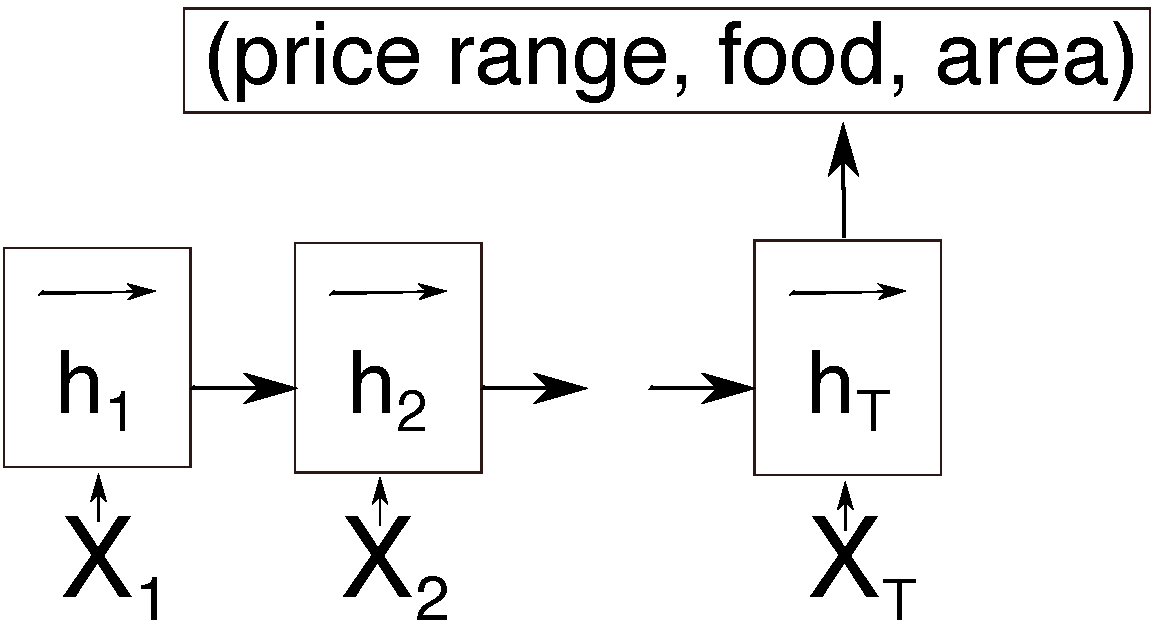
\includegraphics[width=0.5\textwidth]{encoder_joint}
\caption{The joint label predictions using RNN.}
\label{fig:encjoint}
\end{figure}

\subsection{Predicting labels independently}
\label{sec:indep}
Independent slots prediction using one classifier per each slot is also very easy to implement.
It does not suffer from the curse of dimensionality but it introduce unrealistic assumption of uncorrelated slot properties.
In case of DSTC2 and Cambridge restaurant domain it is hard to believe, that slots $area$ and $price range$ do not correlate.
\begin{figure}
\includegraphics[width=0.5\textwidth]{encoder}
\caption{The RNN encodes the word history into dialog state $h_T$ and predicts slot values independently.}
\label{fig:encind}
\end{figure}

\subsection{Encoder decoder framework}
\label{sec:encdec}
The encoder decoder model with attention\cite{bahdanau2014neural} is the most sophisticated model we used for slot predictions.
To our knowledge, we are first who used this model for the task of slot predictions.
The model is typically used in machine translation,since it's able to handle longer sequences with good accuracy and it captures correlation between decoded slots easily\cite{bahdanau2014neural}.

The disadvantage of this model is its complexity.
Firstly, the model is not straightforward to implement\footnote{We modified code from TensorFlow `seq2seq` module.}. Secondly, the decoding time is quadratic in length of the decoded tuples.
However, it is trivial to encode dialog state tracking as sequence-to-sequence problem. Given the the dialogue history as input sequence we trained the model to predict always four labels representing the first, the second, the third slot and end of string symbol.
Since our target sequence is always of length four the model does not suffer from long decoding time.
\begin{figure}
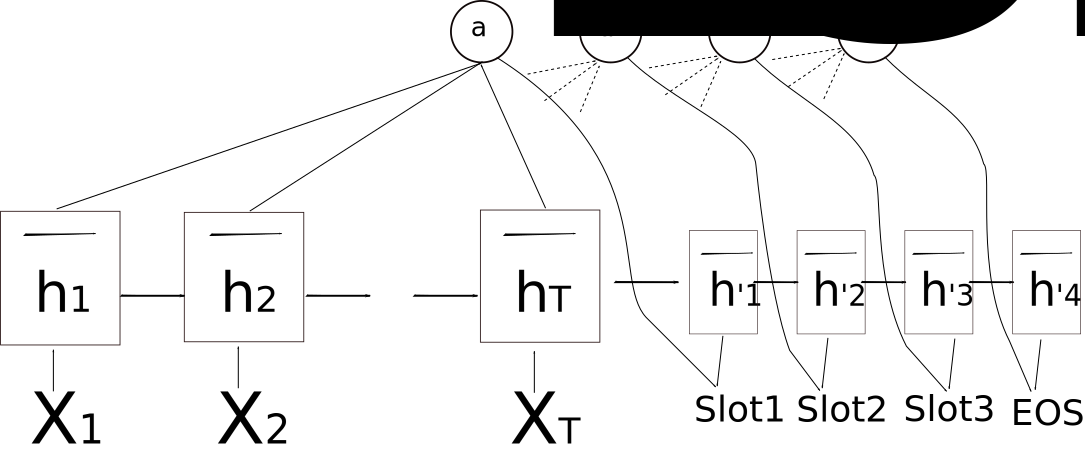
\includegraphics[width=0.5\textwidth]{encdec}
\caption{Encoder decoder with attention predicts goals.}
\label{fig:encdec}
\end{figure}

\section{Experiments}
\label{sec:exp}
We report results on the standard split where we used 10\% of data from $train\_dev$ data as a validation set for early stopping\cite{prechelt1998early} and 90\% for training.
The joint slot accuracy is predicted from \OP{VERIFY GOLD OR ASR transcription only}.
We report accuracy  on development set which we created and official test set. See~Table~\ref{tab:dstc}.
% \todo{nechceme reportovat i train a valid? me to vetsinou v clancich zajima} muzem kdyz to stihnem, ale validace na trenovani trva dlouho a nechce se mi to prepocitavat na validacni sade to mame

For all our experiments, we train word embeddings of size 100, use encoder state size of size 100 together a dropout constant keep probability of 0.7 for both encoder inputs and outputs.
These parameters where selected after grid search on the parameters.
% Me to prijde nepodstatne, ja jsem zkousel od 30 po 300 a 100 mi vysel nejlepsi, zduvodnil jsem to grid searchem a experimenty.\PB{Navic bych pripsal: The common embedding dimension is commonly selected much higher in machine translation but in order to limit the model variance we decided to decrease the number of trainable parameters.} \todo{source}

\subsection{Training}
\label{sec:train}
The training is optimized using the cross-entropy loss function and Adam optimizer\cite{kingma2014adam} with batch size ten.
We train predicting goal slot values at the end of each turn by feeding to the model the turn slot labels $labels_t$ and the whole dialog history until the turn $t$.
Since the dialog lengths vary a lot and batch our inputs, we separated the dialogues according their lengths into ten buckets to speed up the computation. We reshuffle the data after each epoch only within a bucket.
Early stopping with patience\cite{prechelt1998early} of four models is run after each epoch on validation set.

\subsection{Labels representation evaluation}
\label{sec:eval}
The predicted labels depend often on the dialogue full history and not only last turn which makes the task very challenging.
Our informal experiments showed, that optimizing the training only on last turn\footnote{The prediction was conditioned on full history but we back-propagated the error only in words for last turn.} degrades the performance significantly by more than 40\%.

Predicting the labels jointly is quite challenging because the distribution of the labels is skewed as demonstrated in~Figure~\ref{fig:labels}.
As some of the labels combinations are very rare they occur only in the development and test set so the joint model is not able to predict them.
We think that such data sparsity of slot triples causes the degraded performance of the joint model.

\begin{figure}
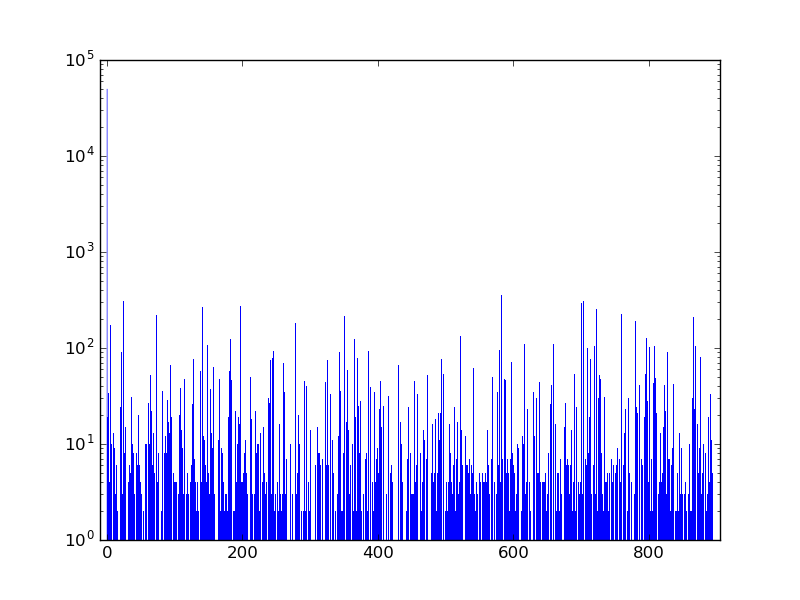
\includegraphics[width=0.5\textwidth]{dstc2_goals_joint_log_scale}
\caption{The log-scaled histogram of joint labels. The x axis represents the id of the $(food, area, pricerange)$ triple.}
\label{fig:labels}
\end{figure}

\OP{VALIDATE THIS PARAGRAPH after experiments update}
The model with independent label prediction obtained much better performance on each slot individually as expected, but also it surprisingly outperformed the joint model in the joint prediction.
We hypothesize that with larger amount of data the joint model would suffer less from data sparsity and perform better.
This claim is supported by comparison of joint and independent models performance on the original DSTC2 dataset.
In this dataset, the training and test set differ much more than on our resplitted version. 
See Table~\ref{tab:dstc} and Table~\ref{tab:resplit} for details.

\begin{table}
\caption{Accuracy on development and {\it Dstc2 test set }}
\begin{center}
\begin{tabular}{r@{\quad}rll}
\hline
\multicolumn{1}{l}{\rule{0pt}{12pt}
                   Model}&\multicolumn{1}{l}{Dev set}&\multicolumn{2}{l}{Test set}\\[2pt]
\hline\rule{0pt}{12pt}
Joint  &     ?&  todo \\
Indep  &   todo& todo \\
EncDec &   0.94 & todo \\
\hline
\end{tabular}
\end{center}
\label{tab:dstc}
\end{table}

Since the encoder decoder architecture is much more general, it needed also to learn how to predict only three slot labels in the correct order.
It turned out, that the architecture learned to predict tuples of four with three slot values and end of string (EOS) symbol quickly even before seeing first half of training data in the first epoch.
At the end of first epoch it made no more mistakes on predicting slot values in the incorrect order.
The encoder decoder strongly outperformed previous models and the time needed for learning the output structure was surprisingly short.\footnote{The best model weights were typically found between fifth and eight epoch for all model configurations including encoder-decoder settings.}

\subsection{Data preparation experiments}
\label{sec:split}
The data for DSTC2 test set were obtained from another system than the data for validation and training set.\cite{henderson2014second}.
We wanted to investigate how this influences the complexity of the dataset so we merge all DSTC2 data together and created splits of 80\%, 10\% and 10\% for training, development and test set.
The results in Table~\ref{tab:resplit} show that the complexity of the task dropped significantly.

\begin{table}
\caption{Accuracy on dev and test set of resplitted DSTC2 data}
\begin{center}
\begin{tabular}{r@{\quad}rll}
\hline
\multicolumn{1}{l}{\rule{0pt}{12pt}
                   Model}&\multicolumn{1}{l}{Dev set}&\multicolumn{2}{l}{Test set}\\[2pt]
\hline\rule{0pt}{12pt}
Joint  &     ?&  todo \\
Indep  &   0.87 & todo \\
EncDec &   0.94 & todo \\
\hline
\end{tabular}
\end{center}
\label{tab:resplit}
\end{table}

\section{Related work}
\label{sec:related}
Our system is related to RNN tracker of \cite{zilka2015incremental}\todo{full-name reference} which reported near state-of-the art result on DSTC2 dataset and was the first incremental system which was able to update the dialog state word-by-word with such accuracy.
In contrast to work of \cite{zilka2015incremental}\todo{full-name reference} we use no abstraction of slot values but we added the additional features as described in Section~\ref{sec:model}.
The first system which used Neural Network for dialog state tracking \cite{henderson2013deep} used feed forward network and manually engineered more than ten features across different levels of abstraction of the user input, including spoken language understanding component (SLU).
In our work we focused on simplifying the architecture and so we used only features which were explicitly given by the dialog history word representation and the database.

The system of \cite{henderson2014word}\todo{full-name reference} gives state-of-the-art results and like our system it predicts the dialog state from words using a recurrent neural networks.
On the other hand, their system heavily relies on user input abstraction.
Another dialog state tracker with LSTM was used in reinforcement setting but they also used information from SLU pipeline.\cite{lee2016dialog}

It is worth noting, that there are first attempts to train end-to-end dialog system even without explicitly modeling dialog state\cite{bordes2016learning} which further simplifies the architecture of a dialog system.
However, the reported end-to-end model was evaluated only on artificial dataset and cannot be compared to DSTC2 dataset directly.

\todo{Tady by stalo za to zminit praci Volodana a dalsich}
\OP{Myslis Vodolana? http://arxiv.org/abs/1510.03710, klidne bych to tam pridal az doladime zbytek clanku a uvidime kolik nam zbyva mista.}

\section{Conclusion}
\label{sec:conc}
% Done \PB{Podle me by to chtělo rozdělit na dva nadpisy}

We presented a dialog state tracking models which represents state of the art models using recurrent neural networks and compare them among each other.
To our knowledge we were the first who used encoder-decoder model for the dialog state tracking task, and we encourage others to do so because it outperformed other standard RNN models.
We also suggest that evaluating dialog state tracking in DSTC2 test set is notoriously hard and that the task become substantially easier if the data are reshuffled.

\subsection*{Future work}
In the future we plan to evaluate the models using standard evaluation metrics on DSTC2 including L2 norm.
We also plan to predict all slots tracked in the DSTC2 dataset.
Another direction of our future work will focus on collecting and annotating data so we would be able to evaluate the models on another task-oriented dataset.


\subsection*{Acknowledgment}
This research was partly funded by the Ministry of Education, Youth and Sports of the Czech Republic under the grant agreement LK11221, core research funding, grant GAUK 1915/2015, and also partially supported by SVV project number 260 224. 
We gratefully acknowledge the support of NVIDIA Corporation with the donation of the Tesla K40c GPU used for this research.
Cloud computational resources were provided by the MetaCentrum under the program LM2010005 and the CERIT-SC under the program Centre CERIT Scientific Cloud, part of the Operational Program Research and Development for Innovations, Reg. no. CZ.1.05/3.2.00/08.0144.


\bibliographystyle{plain}
\bibliography{samplearticle}

% %
% % ---- Bibliography ----
% %
% \begin{thebibliography}{5}
% %
% \bibitem {clar:eke}
% Clarke, F., Ekeland, I.:
% Nonlinear oscillations and
% boundary-value problems for Hamiltonian systems.
% Arch. Rat. Mech. Anal. {\bf 78} (1982) 315--333
% \bibitem {clar:eke:2}
% Clarke, F., Ekeland, I.:
% Solutions p\'{e}riodiques, du
% p\'{e}riode donn\'{e}e, des \'{e}quations hamiltoniennes.
% Note CRAS Paris {\bf 287} (1978) 1013--1015
% \bibitem {mich:tar}
% Michalek, R., Tarantello, G.:
% Subharmonic solutions with prescribed minimal
% period for nonautonomous Hamiltonian systems.
% J. Diff. Eq. {\bf 72} (1988) 28--55
% \bibitem {tar}
% Tarantello, G.:
% Subharmonic solutions for Hamiltonian
% systems via a $\bbbz_{p}$ pseudoindex theory.
% Annali di Matematica Pura (to appear)
% \bibitem {rab}
% Rabinowitz, P.:
% On subharmonic solutions of a Hamiltonian system.
% Comm. Pure Appl. Math. {\bf 33} (1980) 609--633
% \end{thebibliography}



\end{document}
